\section{Zielsetzung}
\label{sec:Zielsetzung}
Das Ziel des Versuchs ist die Beschäftigung mit der Charakteristik eines Geiger-Müller- 
Zählers. Dazu wird die Kennlinie der Stoffes \ce{^{204}Tl} analysiert und 
die Totzeit des verwendeten Geiger-Müller-Zählrohrs bestimmt.
\section{Theorie}
\label{sec:Theorie}
\subsection{Aufbau und Funktion des Zählrohrs}
Das Geiger-Müller-Zählrohr wird zur Messung von $\alpha$-, $\beta$- 
und $\gamma$- Strahlung verwendet. Allerdings ist die 
Nachweiswahrscheinlichkeit für $\gamma$ Strahlung sehr gering, weshalb das Zählrohr
hauptsächlich zur Messung von $\alpha$ und $\beta$ verwendet wird. $\alpha$-Strahlung 
besteht aus Heliumkernen, die $\beta⁺$ Strahlung besteht aus Positronen, die
$\beta⁻$- Strahlung besteht aus Elektronen und die $\gamma$-Strahlung ist energiereiche elektromagnetische 
Strahlung. Der prinzipielle Aufbau eines Geiger-Müller-Zählrohrs ist in Abbildung (\ref{fig:Aufbau}) zu sehen. 
\begin{figure}[H]
    \centering
    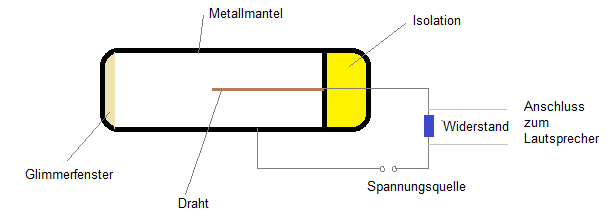
\includegraphics[width=\textwidth]{content/Bilder/Zaehlrohr_Aufbau.png}
    \caption{Schematischer Aufbau des Geier-Müller-Zählrohrs \cite{Aufbau}.}
    \label{fig:Aufbau}
\end{figure}

Das Zählrohr besteht aus einem negativ geladenen, metallischen Zylinder. An einer Seite 
ist der Zylinder durch ein Glimmerfenster verschlossen. In der Mitte des Zylinders ist
auf dessen Achse ein Draht aus Wolfram, der mit einem hochohmigen Widerstand verbunden ist. 
Das Innere des Rohrs ist mit einem Edelgas versetzt mit Kohlenwasserstoff gefüllt. 
Nach dem hochohmigen Widerstand ist das Messrohr mit einem Verstärker verbunden, um die 
vom Rohr erzeugten Spannungsimpulse messbar zu machen. 
Die Funktionsweise des Rohrs wird im Folgenden erläutert. 
Zwischen dem positiven Draht und dem negativ geladenen Zylinder wird ein elektrisches 
Feld angelegt. Wenn ein ionisiertes Teilchen durch das Glimmerfenster in das Zählrohr 
kommt, wird das Gas im Inneren ionisiert. Die entstehenden Elektronen werden 
in die Mitte zum Draht und die positiven Ionen zum Zylinder gezogen und am jeweiligen 
Ort gesammelt. Durch den Energiezuwachs, den die Teilchen durch die Beschleunigung 
erfahren, können diese auf dem Weg weitere Atome ionisieren und dadurch eine Lawine
auslösen. Wenn genug Elektronen sich am Draht gesammelt haben, wird der Widerstand überwunden
und die Spannung fällt schlagartig ab. Dadurch wird die Feldstärke des elektronischen Feldes 
weniger und die Kettenreaktion stoppt. Danach baut sich das elektronische Feld wieder auf. 
Während dieses Vorgangs ist keine weitere Dedektion eines Teilchens möglich. 
 
\subsection{Kennlinie}
Ein Geiger-Müller-Zählrohr hat eine typische Kennlinie, die schematisch in Abbildung 
(\ref{fig:Kennlinie}) zu sehen ist. Die Kennlinie kann in fünf Bereiche aufgeteilt werden. 
Der erste Abschnitt heißt Rekombination. In diesem Bereich ist die Spannung des elektrischen 
Felds noch zu gering, als dass das einfallende Teilchen andere Atome ionisieren könnte. 
Daher bindet das einfallende Teilchen sich mit anderen Atomen zu einem neutralen Teilchen. 
Im zweiten Bereich, der sogenannten Ionisationskammer, ist die Spannung so groß, 
dass die einfallenden Teilchen nicht rekombiniert werden zu neutralen Teilchen, sondern
alle erzeugten Elektronen und Ionen erreichen den Draht bzw. den Zylinder. Diese werden 
allein von der Primärspannung erzeugt. Der sich anschließende Bereich ist der 
Proportionalitätsbereich. In diesem Bereich wird das einfallende Teilchen so stark 
beschleunigt, dass es genug Energie hat, um andere Atome zu Ionisieren. Die daraus 
entstehenden Elektronen erreichen ebenfalls eine so hohe Energie, dass sie 
andere Atome ionisieren können. Diese entstehenden Lawinen werden Townsend-Lawinen genannt 
und treten nur örtlich begrenzt auf. Die Lawinen führen zu einer Verstärkung des 
Signals um ungefähr $10³$. Innerhalb dieses Bereiches kann das dedektierte Teilchen 
nach Art und Energie unterschieden werden, da $\alpha$- und $\beta$-Teilchen und $\gamma$-Strahlung 
unterschiedlich viele freie Ladungsträger im Rohr produzieren.  
\begin{figure}[H]
    \centering
    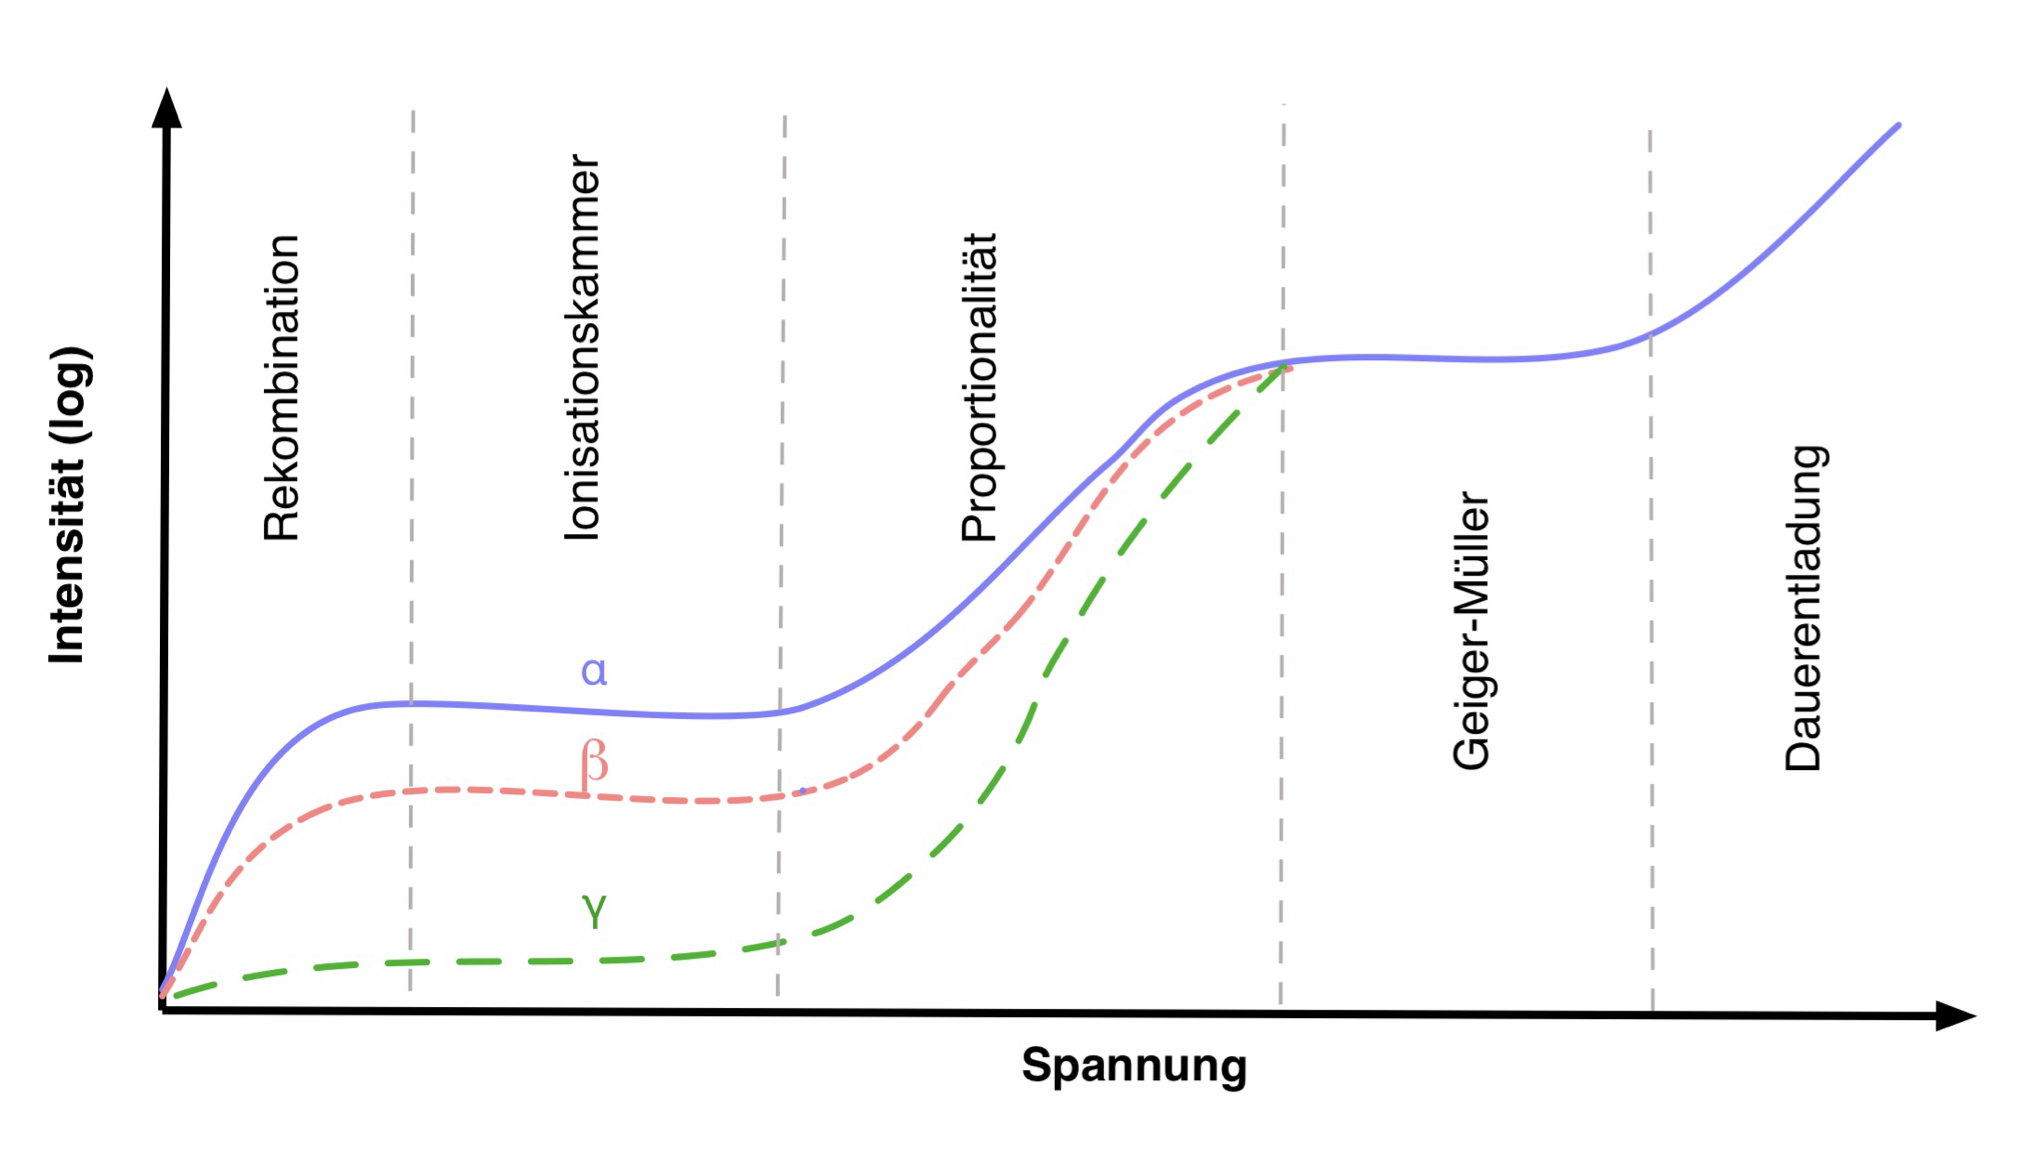
\includegraphics[width=\textwidth]{content/Bilder/Kennlinie.jpeg}
    \caption{Kennlinie eines Geier-Müller-Zählrohrs \cite{anleitungV703}.}
    \label{fig:Kennlinie}
\end{figure}
An den Proportionalitätsbereich schließt der Geiger-Müller-Bereich an. In diesem Bereich 
kann anhand des ausgehenden Signals nicht mehr unterschieden werden, welches Teilchen 
eingefallen ist. Anstatt nur lokal begrenzt bilden sich nun im gesamten Rohr Lawinen aus, 
Die dadurch entstehenden Elektronen fließen über den Anodendraht ab, die massereicheren und daher 
trägeren Atomrümpfe bilden allerdings um den Draht herum eine positive Ladung und unterdrücken
dadurch das Ausbilden weiterer Lawinen. Bei der Höhe der Spannung, die das elektrische 
Feld im Geiger-Müller-Bereich hat, können Gasatome nicht nur ionisiert, sondern auch 
angeregt werden. Dies führt dazu, dass diese Photonen emittieren können, die wiederum in 
der Kathodenwand des Metallzylinders Elektronen auslösen können. Diese Elektronen werden
im elektrischen Feld beschleunigt und führen zur Lawinenbildung. Um diese Störung der
Messung zu vermeiden, ist die Innenseite des Zylinders mit Löschalkohol beschichtet, welcher
die Photonen absorbiert und dadurch ein Auslösen weiterer Elektronen verhindert. Der 
letzte Bereich ist der Bereich der Dauerentladung. In diesem Bereich führt die hohe Spannung
zur Dauerentladung, welche das Messgerät zerstören kann.  

\subsection{Güte des Zählrohrs}
Das Maß für die Güte des Zälrohrs ist die Steigung des Plateaus im Geiger-Müller-Bereich. 
Diese entsteht dadurch, dass nicht jeder Elektronenausschlag aus dem Zylinder durch den 
Löschalkohol verhindert werden kann und durch diese Elektronen zeitlich versetzte 
Ausgangsimpulse entstehen. Diese Impulse stellen eine Verfälschung des Ergebnisses dar und 
führen dazu, dass das Geiger-Müller-Plateau eine positive Steigung $s$ hat. Es gilt 
\begin{equation}
    s = \frac{\Delta N}{N} \cdot \frac{100 \,\%}{100 \unit{\volt}} \, .
    \label{eqn:s_anderes}
\end{equation}
In dieser Formel ist $\frac{\Delta N}{N}$ die relative Zählrate und $s$ ist pro 
$100 \unit{\volt}$ Spannungsänderung definiert. Wenn der Arbeitspunkt $U_A$ bekannt ist, 
kann auch die Formel 
\begin{equation}
    s = \frac{\left(U_A + 50 \, \unit{\volt}\right) - \left(U_A - 50 \, \unit{\volt} \right)}{U_A}
    \label{eqn:s_arbeitspunkt}
\end{equation}
verwendet werden.
\subsection{Totzeit}
In der Zeit, in 
der sich die positive Ladungswolke um den Draht herum gebildet hat, ist das Messgerät
nicht in der Lage ein weiteres Teilchen zu Dedektieren. Erst nach Abfließen der Ladung
und Aufbau des Feldes kann ein neues Teilchen gemessen werden. Dieses Zeitintervall
heißt Totzeit. Während sich das elektrische Feld wieder aufbaut können Teilchen gemessen 
werden, das ausgehende Signal ist allerdings kleiner als sonst. Diese Zeit heißt
Erholungszeit. Totzeit und Erholungszeit können auf dem Oszilloskopbild abgelesen werden,
wie in Abbildung (\ref{fig:Totzeit}) zu sehen. 
\begin{figure}[H]
    \centering
    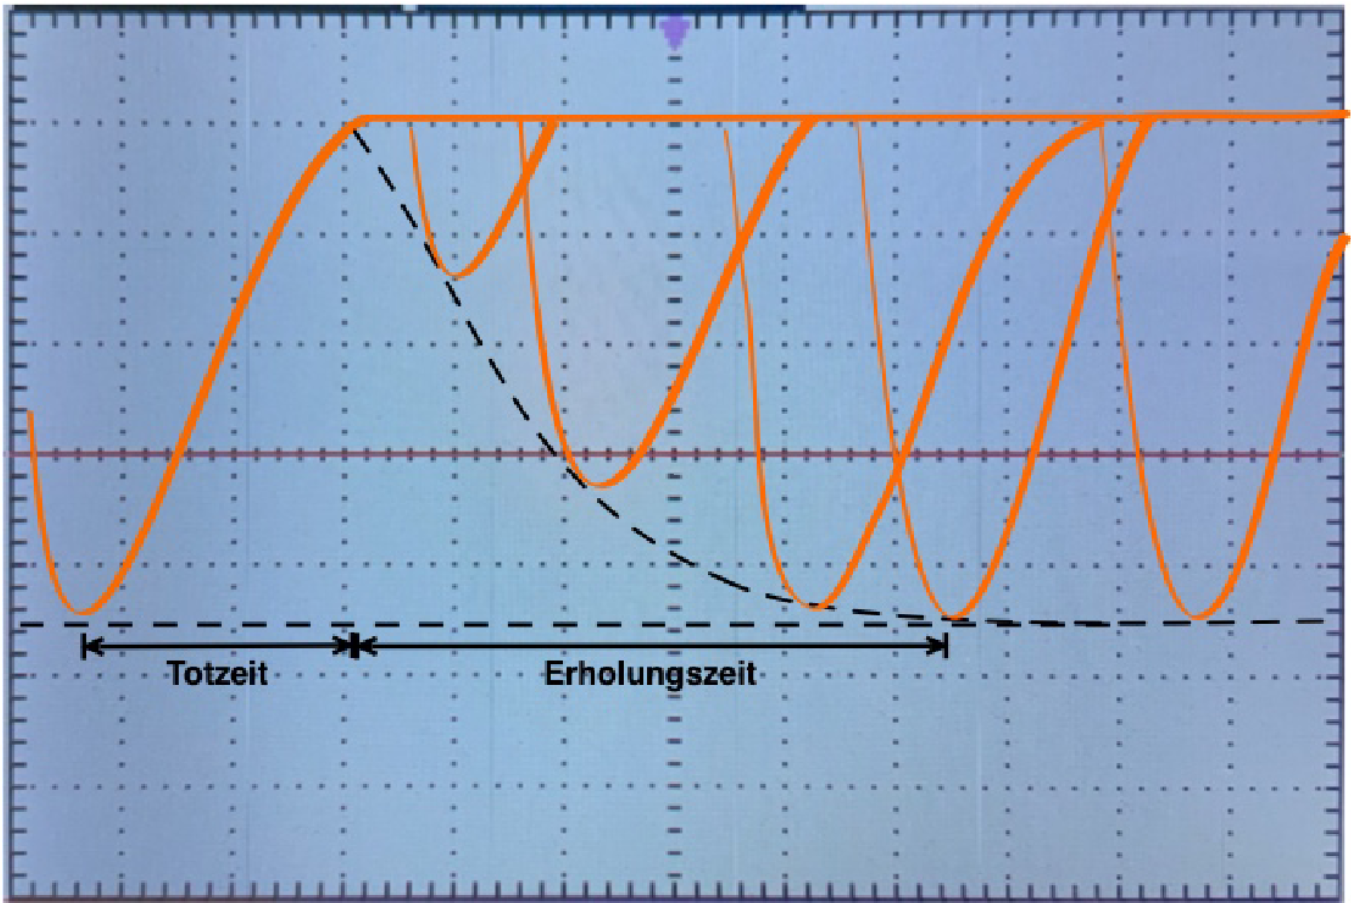
\includegraphics[width=\textwidth]{content/Bilder/Oszilloskop.png}
    \caption{Totzeit und Erholungszeit des Geiger-Müller-Zählrohrs \cite{anleitungV703}.}
    \label{fig:Totzeit}
\end{figure}
Die Totzeit kann außerdem mithilfe der Zwei-Quellen-Methode bestimmt werden. Dazu wird die Zählrate 
zwei verschiedener Quellen erst einzeln gemessen ($N_1$ der ersten Quelle und $N_2$ der zweiten Quelle).
Anschließend wird die Zählrate $N_{12}$ beider Quellen zusammen gemessen. Die Totzeit $\tau$
lässt sich dann mithilfe von 
\begin{equation}
    \tau = \frac{N_1 + N_2 - N_{12}}{N_{12}² - N_1² - N_2²}
    \label{eqn:tau_tilde}
\end{equation}
berechnet werden.
\subsection{Vorbereitungsaufgaben}
\label{sec:Vorbereitungsaufgaben}
Zur Vorbereitung wird die Halbwertszeit und die Zerfallskanäle von \ce{^{204}Tl}
recherchiert. Die Halbwertszeit beträgt $3,783$ Jahre und \ce{^{204}Tl}
zerfällt zu $2,92 \, \%$ durch einen $\beta⁺$ in \ce{^{204}Hg} und zu $97,08 \, \%$ 
durch einen $\beta⁻$ Zerfall in \ce{^{204}Pb} \cite{vorbereitung}. 
Außerdem sollte die Zährate $N \geq 10.000$ sein, um eine statistische Messunsicherheit
von $1 \, \%$ zu erhalten, da die statistische Messunsicherheit proportional zu 
$\sqrt{N^{-1}}$.
